\chapter{Considerações}
\label{ch:consideracoes}

De um modo geral, a maioria das pesquisas em algoritmos evolutivos concentra-se em problemas de otimização estáticos. No entanto, muitos problemas do mundo real são problemas de optimização dinâmica, em que as mudanças ocorrem ao longo do tempo. Isso requer algoritmos de otimização, não só para encontrar a solução ideal global sob um ambiente específico, mas também para monitorar continuamente a mudança em diferentes ambientes dinâmicos. Assim, são necessários métodos de optimização que são capazes de se adaptar continuamente para um ambiente em mudança.

Os algoritmos de inspiração biológica, em principal, os algoritmos de inteligência de enxame são amplamente estudados para melhorar sua performance em ambientes dinâmicos e com isso vários operadores evolutivos são gerados e aplicados em diferentes problemas dinâmicos com diferentes propriedades. Cada um desses operadores possuem pontos fortes e fracos nas suas aplicações, então o estudo comparativo para identificar esse pontos se faz necessário, de modo que a aplicação em conjunto desses operadores pode se benéfico para ambos, neutralizando esses pontos negativos.

O trabalho até aqui contribui exatamente nesse estudo comparativo das técnicas de otimização em ambientes dinâmicos. Nos estudos feitos até agora pode-se notar uma grande quantidade de operadores evolutivos e suas influências, de modo que a aplicação desses operadores no FSS pode ser esquematizada para que, na próxima etapa do trabalho, seja concluída. Os métodos de manutenção da diversidade populacional contribuem em geral na otimização dos ambientes dinâmicos com domínio contínuo pelo fato de que uma alta diversidade contribui na manutenção do nível de \textit{fitness}.

Dado o desenvolvimento do Trabalho de Conclusão de Curso até o momento, é apresentado neste trabalho as próximas etapas a serem desenvolvidas pelo cronograma até o final do trabalho:

\subsubsection{Cronograma}
\label{sec:cronograma}

\begin{enumerate}
\item Analisar a influencia dos operadores encontrados e avaliar quais devem ser aplicados no algoritmo;
\item Desenvolver a versão definitiva do algoritmo utilizando todos os operadores evolutivos alternadamente;
\item Experimentos computacionais com o algoritmo e os problemas selecionados;
\item Coleta e análise dos resultados dos experimentos; 
\item Finalização da escrita do trabalho de conclusão de curso
\end{enumerate}

\begin{figure}[!htb]
	\caption{Cronograma para o TCC - 2}
	\centering
	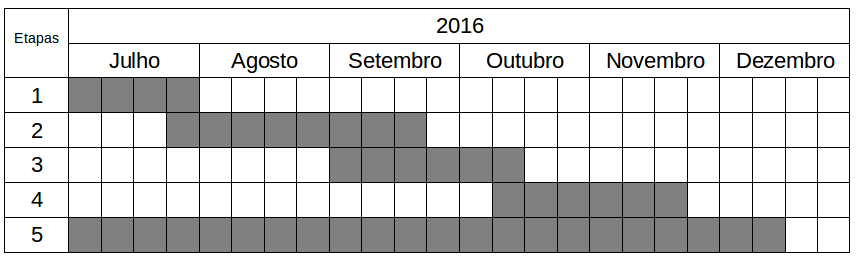
\includegraphics[scale=0.5]{images/cronograma.png}
	\label{fig:cronograma}{\\Fonte: Produção do próprio autor.}
\end{figure}

